\documentclass[prl,aps,twocolumn]{revtex4}
%\usepackage{ctex}
\usepackage{mathrsfs,amssymb,amsfonts,amsmath,bm}
\usepackage{tikz}


%%%%%%%%%%%%%%%%%正体微分%%%%%%%%%%%%%%%%%%
\newcommand*\dd{\mathop{}\!\mathrm{d}}
\newcommand*\ddd[1]{\mathop{}\!\mathrm{d^#1}}
%%%%%%%%%%%%%%%%%%%%%%%%%%%%%%%%%%%%%%%%%

%%%%%%%%%%%%%%%%%%%%%方程按节编号%%%%%%%%%%
%\numberwithin{equation}{section}
%%%%%%%%%%%%%%%%%%%%%%%%%%%%%%%%%%%%%%%%%


\begin{document}
%\draft

\title{Physical Phases Regonition by Machine Learning}
\author{Xiaodong Hu\footnote{PB14203081, \url{cdqz2014@mail.ustc.edu.cn}}, Zhican Chen\footnote{PB14203085}, Yixiao Xi\footnote{PB14210052}}
\affiliation{Department of Modern Physics, University of Science and Technology of China, Anhui, Heifei}
\affiliation{Department of Physics, University of Science and Technology of China, Anhui, Heifei}
\affiliation{Department of Computer Science, University of Science and Technology of China, Anhui, Heifei}
\affiliation{Repository: \url{https://github.com/cdqz2014/Physical-Phase-Recognition-by-Machine-Learning}}
\date{\today}

\begin{abstract}
Ising Model is a well-known toy model in statistical physics and computational physics. As a typical physics model related to phase trainsition and even topological excitations recently, Ising Model has been well-digged for more than fifty years but only in one and two dimensional cases the analytical expressions are obtained. In this article, we utilize both the tools of supervised learning and unsupervised learning to studied the two phases of the two-dimensional Ising model of squared lattice. We first generated the spin configurations by Monte Carlo methods, then developed a shallow but effective neural network and optimized it by making the full-connected network deep. Additionally, we use the celebrated k-means algorithms to cluster the scatter diagrams of magnetization-temperature after manual dimenisonality reduction to obtain the two phases. The coincidence of the boundary of two clusters and the theoretical critical temperature proved our model to be powerful. 
\end{abstract}
%, whose validity is guaranteed by the principle of detailed balence and theorem of Markov chain 

\pacs{}
\maketitle

\section{Data Preparation -- Monte-Carlo Methods}
	%All the interacting and evolving processes in statistical mechanics are \emph{Markov processes}. But a mathematical theorem in stochastic process, we can awalys reach the equilibrim point at arbitrary initial value.
	\subsection{Monte-Carlo Methods}Monte-Carlo methods are a broad class of computational algorithms that rely on repeated random sampling to obtain numerical results. Their essential idea is using randomness to solve problems that might be deterministic in principle. They are often used in physical and mathematical problems and are most useful when it is difficult or impossible to use other approaches. In this project we mainly imply the simplest one: 16807 Random Number Generator to generate large amounts of random numbers ranking from -1 to 1. With the random numbers generated, we could initialize the system at arbitrary value and determine whether or not to flip a particle's spin with Metropolis-Hastings Algorithm introduced below.
    \subsection{Ising model}The Ising model is a mathematical model of ferromagnetism in statistical mechanics. The model consists of discrete variables that represent magnetic dipole moments of atomic spins that can be in one of two states (+1 or −1). The spins are arranged in a graph, usually a lattice, allowing each spin to interact with its neighbors. The model allows the identification of phase transitions, as a simplified model of reality. The two-dimensional square-lattice Ising model is one of the simplest statistical models to show a phase transition.
    \indent Since every spin site has ±1 spin, there are $2^L$ different states that are possible.This motivates the reason for the Ising model to be simulated using Monte Carlo methods.\\
    The Hamiltonian that is commonly used to represent the energy of the model when using Monte Carlo methods is:
    \begin{equation}
      H(\sigma)=-J\sum_{<i,j>}\sigma_i\sigma_j-h\sum_{j}\sigma_j
    \end{equation}

    \begin{figure}[htb]
      \includegraphics[width=0.5\linewidth]{Ising.png}
      \caption{Ising model}
      \label{fig:1}
    \end{figure}
    \indent Given this Hamiltonian, quantities of interest such as the specific heat or the magnetization of the magnet at a given temperature can be calculated. Especially in our Monte Carlo simulation, the Metropolis-Hastings algorithm is the most commonly used Monte Carlo algorithm to calculate Ising model estimations. The algorithm first chooses selection probabilities $g(\mu,\nu)$, which represent the probability that state $\nu$ is selected by the algorithm out of all states, given that one is in state $\mu$. It then uses acceptance probabilities $A(\mu,\nu)$ so that detailed balance is satisfied. If the new state $\nu$ is accepted, then we move to that state and repeat with selecting a new state and deciding to accept it. If $\nu$ is not accepted then we stay in $\mu$. This process is repeated until some stopping criterion is met, which for the Ising model is often when the lattice becomes ferromagnetic, meaning all of the sites point in the same direction.
    \indent Since there are L total sites on the lattice, using single-spin-flip as the only way we transition to another state, we can see that there are a total of L new states $\nu$ from our present state $\mu$. The algorithm assumes that the selection probabilities are equal to the L states: $g(\mu,\nu) = 1/L$. Detailed balance tells us that the following equation must hold:
    \begin{equation}
      \frac{P(\mu,\nu)}{P(\nu,\mu)}=\frac{g(\mu,\nu)A(\mu,\nu)}{g(\nu,\mu)A(\nu,\mu)}=\frac{\frac{1}{Z}e^{-\beta(H\nu)}}{\frac{1}{Z}e^{-\beta(H\mu)}}=e^{-\beta(H\nu-H\mu)}
    \end{equation}
    Thus, we want to select the acceptance probability for our algorithm to satisfy:\\
    \begin{equation}
    \frac{A(\mu,\nu)}{A(\nu,\mu)}=e^{-\beta(H\nu-H\mu)}
    \end{equation}
    If $H\nu > H\mu$, then $A(\nu, \mu) > A(\mu, \nu)$ \\\\
    Metropolis sets the larger of $A(\nu, \mu)$ or $A(\mu, \nu)$ to be 1. By this reasoning the acceptance algorithm is:
    \begin{equation}
      A(\mu,\nu)=\left\{
                 \begin{aligned}
                      & e^{-\beta(H\nu-H\mu)}, & \text{if}\quad H\nu-H\mu >0 \\
                      & 1,                     & \text{otherwise} \\
                 \end{aligned}
                 \right.
    \end{equation}
    The basic form of the algorithm is as follows:
    \begin{itemize}
      \item Pick a spin site using selection probability $g(\mu,\nu)$ and calculate the contribution to the energy involving this spin.
      \item Flip the value of the spin and calculate the new contribution.
      \item If the new energy is less, keep the flipped value.
      \item If the new energy is more, only keep with probability $e^{-\beta(H\nu-H\mu)}$
      \item Repeat
    \end{itemize}
    The change in energy only depends on the value of the spin and its nearest graph neighbors. So if the graph is not too connected, the algorithm is fast. This process will eventually produce a pick from the distribution.
    \subsection{Physical Explanation}

    In this section, we will prove that this simulation accords with the real physical phenomenon. Firstly, it is important to understand the physical essence we try to describe with the model.
    \paragraph{NVT Ensemble}The principal thermodynamic variable of the canonical ensemble, determining the probability distribution of states, is the absolute temperature (symbol: T). The ensemble typically also depends on mechanical variables such as the number of particles in the system (symbol: N) and the system's volume (symbol: V), each of which influence the nature of the system's internal states. An ensemble with these three parameters is sometimes called the NVT ensemble.
    \indent It is obvious that the Ising model we use accords with all the qualities of NVT Ensemble. To be more specific, the temperature T is fixed to our intended value; the volume V is an $L\times L$ square lattice and the number N is apparently $L^2$.
    \indent According to the qualities of NVT ensemble, we know that the system would eventually reach the equilibrium point at arbitrary initial value. Therefore, we could be saved from the puzzle concerning the initial value setting. Since the initial value wouldn't affect the eventual destination of the system, we could by all means set any value as we wish. Typically in this project, we designate this mission to Monte Carlo method as well.
    \paragraph{Markov Process and Detailed Balance Equations} Previously we have proven that the Ising model we use can be classified as NVT ensemble. However, this doesn't necessarily guarantee the feasibility of our Monte Carlo simulation and Metropolis-Hastings algorithm. Therefore, we have to make sure that whole process can be classified as Markov process.
    \indent Roughly speaking, a Markov process satisfies the Markov property if one can make predictions for the future of the process based solely on its present state just as well as one could knowing the process's full history, hence independently from such history. For instance, the NVT ensemble we describe with Ising model's developing process can be classified as a Markov process. Normally we use the Detailed Balance Equations to judge if a process can be classified as Markov process or not. Luckily, the State Transition Matrix (STM) of Ising model also meets the requirement of detailed balance equations:
    \begin{equation}
    P_1W(1\rightarrow2)=P_2W(2\rightarrow1)
    \end{equation}
    where $P_1$,$P_2$ corresponds to the probability of two microstate when the system reaches equilibrium state.
    To prove this would require large amounts of time and space. Considering that this is not the focus of our work, we hereby simply give the conclusion and omit the details concerning the prove.
    \indent This detailed balance requirement thoroughly guarantees that the simulation method we use could be classified as a Markov process, thus makes sure it accords with the real physical phenomenon. Therefore, we could claim that, after efficient Monte Carlo steps (we would discuss the exact number in the report), this system would definitely reaches thermodynamic equilibrium.
    \subsection{Application: Hopfield Neural Network Model}
    \indent One of the significant properties of the Ising model is: with the evolution of the system, its energy will be reduced spontaneously. As a result, we can design a micro evolution mechanism, which makes the macroscopic functions (such as energy) to be optimized can be naturally optimized. This is the origin of the Hopfield network model.
    \indent Hopfield network is a well-known neural network model. By training the network, it can make it memorize the corresponding patterns, and extract relevant patterns from associative memories under appropriate conditions. That is to say, by training (changing the weight of interconnections), the Hopfield model can map the memory pattern to the smallest energy state, and then evolve to the minimum energy state through the neighborhood interaction rule of the Ising model. A weighted network is shown in FIG 2: each node is a neuron, and the weighted connected side represents the synaptic connection between neurons.
    \begin{figure}[htb]
      \includegraphics[width=0.5\linewidth]{Hopfield.png}
      \caption{Hopfield Neural Network Model}
      \label{fig:2}
    \end{figure}
    It is assumed that each neuron has two states: activation and inactivation, respectively. We use $s_i=+1, -1$ to represent them, and we use $w_{ij}$ to represent the connection weight from neuron i to neuron j. Initially, we map the input vectors to the states (active or inactive) of each neuron. Then, the running rules of the Hopfield network are as follows. In each of the simulation cycles, each neuron updates the state according to the following rules:
    \begin{equation}
        s_i(t+1)=\left\{
			\begin{aligned}
				& 1, & \text{if}\quad\sum_jw_{ij}s_j(t) >\theta_i \\
				& -1,& \text{otherwise} \\
			\end{aligned}
			\right.
    \end{equation}
    According to this rule, if all neurons adjacent to the neuron i are activated and their connection weights are positive, the neuron may be activated. This is the equivalent of minimizing a global energy function, which is defined as:
    \begin{equation}
      E_{{s_i}} = -\sum_{ij}w_{ij}s_is_j - \sum_i\theta_is_i
    \end{equation}
    Then, the Hopfield network running according to the above rules will make the total energy as low as possible. Compared with the Ising model, we see that the energy function of Hopfield is very similar to that of the Ising model, and the difference is that the interaction strength varies with the connection ($w_{ij}$). At the same time, the external field $\theta_i$ is also different because of different neurons. Therefore, the Hopfield network can be regarded as a variant of the Ising model.
    \indent In addition, it is necessary to train the network to make the Hopfield network complete associative memory. Suppose we want the Hopfield network to remember a set of specific vectors (e.g. $V_1, V_2, V_3,\ldots, V_m$), where m is the number of vectors to be learned. Each vector can be written as:
    \begin{equation}
      V_i=<1,-1,1,\ldots,1>
    \end{equation}
    We conciliation weight according to the following rules (where $V_{\nu}(i)$ represents the i component of the vector $\nu$ to be learned):
    \begin{equation}
      w_{ij}=\sum_{\nu=1}^mV_{\nu}(i)V_{\nu}(j)
    \end{equation}
    After training the entire network in this way, we get a set of weights $w_{ij}$. After that, we use these weights as the connection weights in Hopfield network. Then, for any input data as the initial state of neurons, according to the operation rules of Hopfield, the system will gradually converge to one of the memorized vector.
    \indent In summary, the operation of the Hopfield network is divided into two stages, and the intent of their input number is shown in FIG 3.
    \begin{figure}[htb]
      \includegraphics[width=0.8\linewidth]{Hopfield_operating.png}
      \caption{Hopfield Operating Sketch Map}
      \label{fig:3}
    \end{figure}


\section{Supervised Learning of Phase Recognition}
	\subsection{Shallow Effective Neural Network}
		Since Our system has merely two phases, it is natural to believe that a shallow NN will be effective enough. So we built one hidden layer activated by \texttt{Relu} with only two neurons, following by a output layer activated by \texttt{Sigmoid} since the output value is binary: magnetized or not.\par
%		\begin{figure}[!htp]
%			\includegraphics[scale=0.12]{graph-effective.png}
%			\caption{{\bf Shallow Neural Network}.}
%			\label{fig:2.1}
%		\end{figure}
		Though converging little slowly, the training and testing results shown in FIG. \ref{fig:2.1} did prove the effectiveness of this shallow toy model:
		\begin{figure}[!htp]
			\includegraphics[scale=0.16]{effective-test.png}
			\includegraphics[scale=0.16]{effective-training.png}
			\caption{{\bf Losses and Accuracy of Both Training and Test Set for Data of Lattice Size 20}.}
			\label{fig:2.1}
		\end{figure}
		One can observe that the accuracy of the model reaches to exactly one at about $110$ training epoches (with mini-batch $2$).

	\subsection{Deep Neural Network}
		To accelerate the convergence rate, we generalize the shallow NN to a deeper one by expanding the nodes of layer one from two to ten and added another five nodes hidden layer. The structure is shown in FIG. \ref{fig:2.2}:\par
		\begin{figure}[!htp]
			\includegraphics[scale=0.1]{graph.png}
			\caption{{\bf Structure of Our two hidden layers deeper NN}.}
			\label{fig:2.2}
		\end{figure}
		After this slight change, the improvement of the convergence rate of accuracy curve impressioned us that it reaches the exact one at  about only $30$ steps. The comparison of the performance of these two models are drawn in FIG. \ref{fig:2.3} (of course with the same lattice size, mini-batch, and training epoches). 
		\begin{figure}[!htp]
			\includegraphics[scale=0.16]{20-accuracy-compare.png}
			\includegraphics[scale=0.16]{20-training-compare.png}
			\caption{{\bf Comparison of the Training Losses and Testing Accuracy of the Data of Lattice Size 30}. The shallow blue and orange lines represent the losses and accuracy of training data and test data of effective shallow NN while the other two line represent the losses and accuracy of deeper  NN.}
			\label{fig:2.3}
		\end{figure}
		It can also be seen from the distribution diagram FIG .\ref{fig:2.4} that the utilization of every nodes in the Deeper NN is higher than those in shallow effective ones.
		\begin{figure}[!htp]
			\includegraphics[scale=0.18]{20-effect-distribution.png}
			\includegraphics[scale=0.18]{20-distribution.png}
			\caption{{\bf Comparison of the Distribution Diagram of Each Layers}.}
			\label{fig:2.4}
		\end{figure}		
	\subsection{Conclusion}
		In fact, we have also tried to add more layers as well as nodes in our fully-connected neural networks, but the acceleration of the convergence rate improves little. Conversely we have to spend lots of time on the training processes (it's valuable to mention that both these two NN we wrote here cost less than two seconds for one thousand $900$-dimensional vectors). Hence we concluded that sometimes a slight expanding of NN may amazingly upgrade the performance of it.

\section{K-Means Clustering of Phases}
	Although the above neuron network models perform well in physics phase recognization, it demands physics knowledge to obtain the $y$-label for each spin configuration, namely, the magnetization $M$
	\begin{equation}
		M:=\sum_i\dfrac{\sigma_i}{N}.
	\end{equation}
	But \textbf{our target is to develop a general physics phase recognition model to discove phases that theoretical physicists has not predicted and experimentalists has not observed yet}. So A unsupervised learning model, rather than supervised full-conncted NN, is demanded to undertake this task.\par
	But the problem is, if we utilize the flattened data in fully-connected NN in k-means algorithm, then the dimensionality will reach as high as $900$, which will cost large amounts of computational resources and is impossible for us to get the result, let along the number of files for each lattice size is $1000$. In other words, $1000$ points placed in the $900$-dimensional spcace are waited to be clustered.\par
	\hfill\par
	So \textbf{our difficulty is to reduce the dimensionality of spin configuration}. And foutunately we found one the simplest: \par
	Let's start with the simple two-dimensional case. Note that the magnetization is always no less than zero after we manually selecting the magnetization direction (which has no physical meaning), point, i.e., spin configuration $(1,1)$ is farther away from $(-1,-1)$ than $(1,-1)$ does, which exactly coincide the order of the sum of each point. Similar results also holds in three-dimensional case: point $(1,-1,1)$ is farther away from $(-1,-1,-1)$ than $(-1,-1,1)$ does. Generally, we can reshape the high-dimensional data to merely two dimensional through this mapping, \textbf{sum of spin} and \textbf{temperature}.\par
	One may debt that the dimensionality-reduction function here has the similar form of the physical knowledge, namely, the definition of magnetization. But in fact, what motivated us is just the characteristic distrubution of the spin configuration and the partial order relation. We ascribe the similar results to totally coincidence...\par
	Here are the amazing results\par
	\begin{figure}[!htp]
		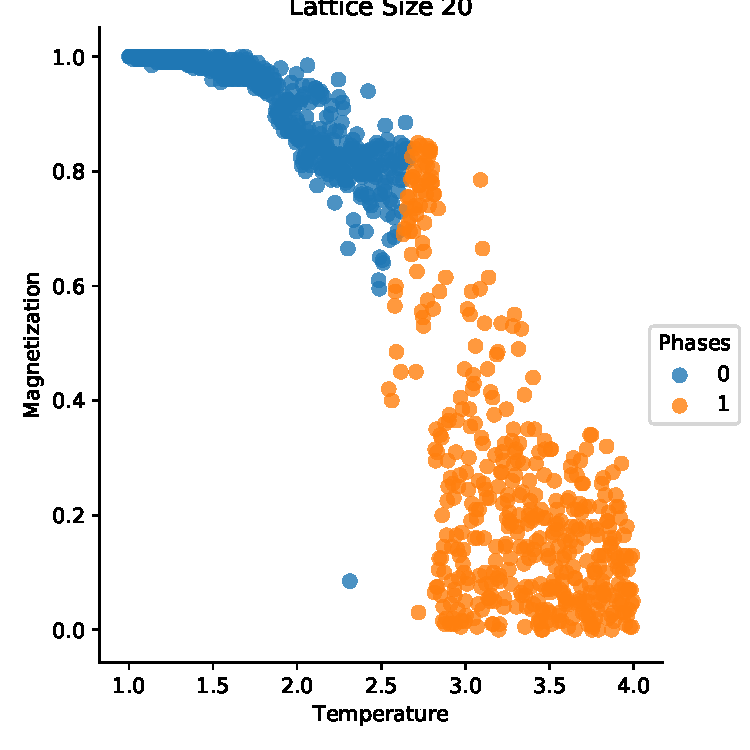
\includegraphics[scale=0.6]{20-1000.pdf}
		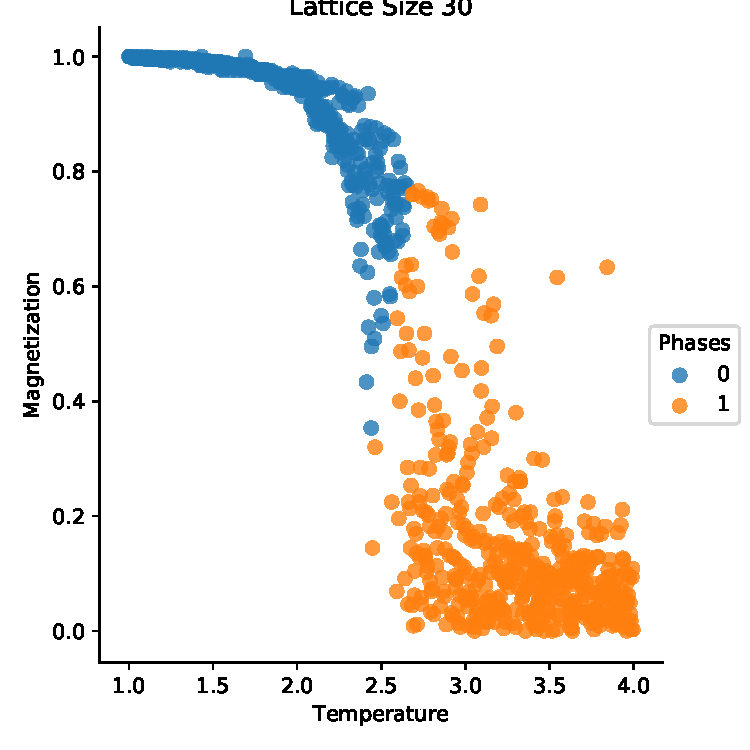
\includegraphics[scale=0.6]{30-1000.pdf}
	\end{figure}
	\begin{figure}[!htp]
		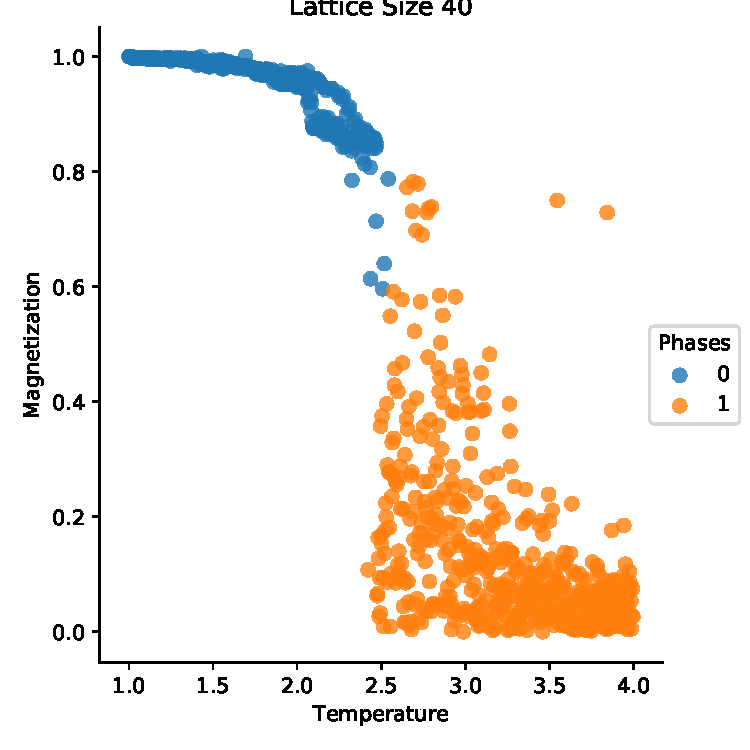
\includegraphics[scale=0.6]{40-1000.pdf}
		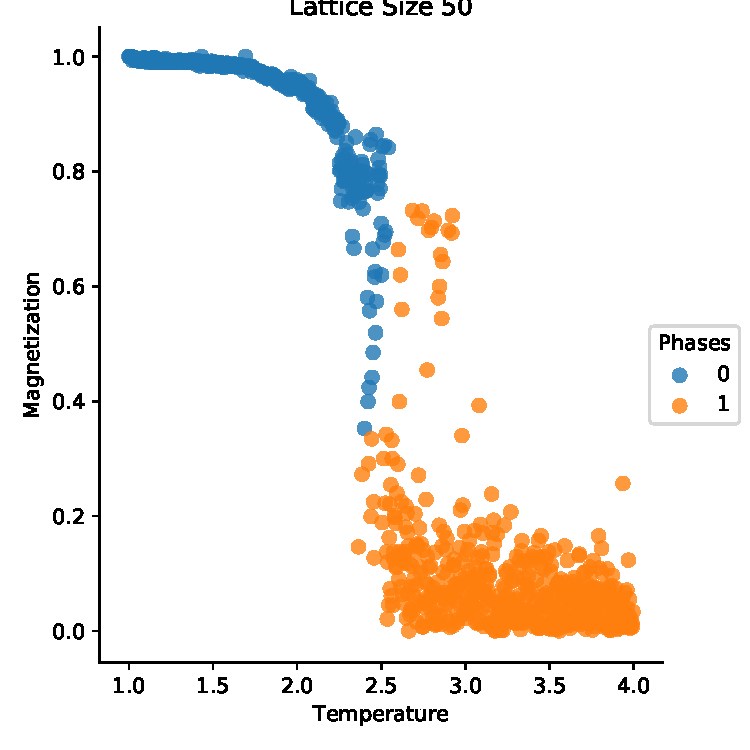
\includegraphics[scale=0.6]{50-1000.pdf}
		\caption{{\bf k-Means Clustering of Lattice Size 50 Data}.}
	\end{figure}
	What surprised us are that not only the k-means algorithm faultlessly divided the $M-T$ figures for different sizes into high-temperature and low-temperature phases, it also gave the more correct \textbf{critical temperature} for phase transition in 2-D Ising model, about $2.25 \mathrm{k}$. As a comparison, theoretical prediction at the \textbf{Thermodynamic Limit} gives
	\begin{equation}
		T_c=\dfrac{2}{\ln(1+\sqrt2)}\approx2.269\,\mathrm{k}
	\end{equation}
	\subsection{Conclusion}
		Another strange thing is, in our k-means algorithm, the initial vector is randomly set, but the clusering results seem surprisingly \textbf{robust} that they always reached the correct recognition of the high-$T_c$ phase and low-$T_c$ phase. In light of the characteristic of the \textbf{second order phase transition} that the dirivatives of the parameter order is not continuous and the crux of the algorithm of k-means that center of mass is ``continuously'' moving, we then audaciously claimed that, \textbf{if a physical system has a second order phase transition, then the clustering result of k-means algorithm is robust}.
	
\section{Training Discussion}
	In this section, we demonstrate some knowledge aquired from training and testing neural network.
	\subsection{Choosing of Activation Function}
		As is shown above, since our NN is not large, the polyline-shaped \texttt{Relu} function makes both the loss curve and accuracy curve also foled. Then it was natural for us to suspect whether it was the activation function \texttt{Relu} that cause those noticable and irregular peaks at large training epoches (which has be smoothed by Tensorboard). So we also tried the recommended \texttt{Tanh} activation function as well. However, the results showing below proved out conjucture to be flase: 
	\begin{figure}[!htp]
		\includegraphics[scale=0.16]{20-tanh-acc.png}
		\includegraphics[scale=0.16]{20-tanh-loss.png}
		\caption{{\bf Accuracy and Losses of the Lattice Size 30 Data}. All polyline-shaped activation functions are replaced with \texttt{Tanh}.}
	\end{figure}

	\subsection{Appropriate Choice of Mini-batch and Epoch}
	To eliminate the strange peaks in both curves, we also tried to change the mini-batch, from one to ten. And fortunately the results in FIG. \ref{fig:3.2} showed that a suitable size of mini-batch will prominently reduce both the heights and number of strange peaks.
	\begin{figure}[!htp]
		\includegraphics[scale=0.16]{batch-acc.png}
		\includegraphics[scale=0.16]{batch-loss.png}
		%\includegraphics[scale=0.2]{color.png}
		\caption{{\bf Accuracy and Losses of the four different Lattice Sizes Data}. Orange and light blue represent the data whose batchsize equals one, i.e., Stochastic Gradient Descending Methods. One can see that SGD, though the quickest, also unfortunately possesses the highest peaks. Conversely, the data whose batch size equals ten has the lowest strange peaks.}
		\label{fig:3.2}
	\end{figure}


	\subsection{Performance under Thermodynamic Limit}
		\textbf{Thermodynamic Limit} is a crucial concept in statistical physics that the rigorous establishment of many theoretical results depend on it. For example, the critical temperature we propose above is under this ideal condition, so this can to some extent explain the slight deviation of our k-means results with the analytic expression. But more interestingly, not only the lattice size influences the establishment of physical laws such as renormalization groups and divergence behavior of the heat capacity, it also influences the training and testing results of the neural network. To put is more explicitly, with the lattice size goes to infinity, the renormalization group reach closer and closer to the unstable critical point, namely, the phase trainsition point. Analogously, we observed that the convergence rate upgraded with the lattice size becaming larger, as is showning in FIG. \ref{fig:3.1}.\par
	\begin{figure}[!htp]
		\includegraphics[scale=0.16]{5-acc.png}
		\includegraphics[scale=0.16]{5-loss.png}
		\includegraphics[scale=0.2]{batch-color.png}
		\caption{{\bf Accuracy and Losses of the Lattice Sizes 30 Data for Different Batches}.}
		\label{fig:3.1}
	\end{figure}
	Mathematically, this phenomenon seems hard to understand, since with the lattice size became larger, the number of parameters in NN also grow as $\mathcal{O}(n^2)$, which should brings more errors and deviations. But if we take the view of physics, then the upgrading of convergence rate can be well-explained.


\bibliographystyle{apsrev}

\end{document}